\chapter{The Go Runtime On Bare Metal}

\begin{figure}[h]
\begin{center}
  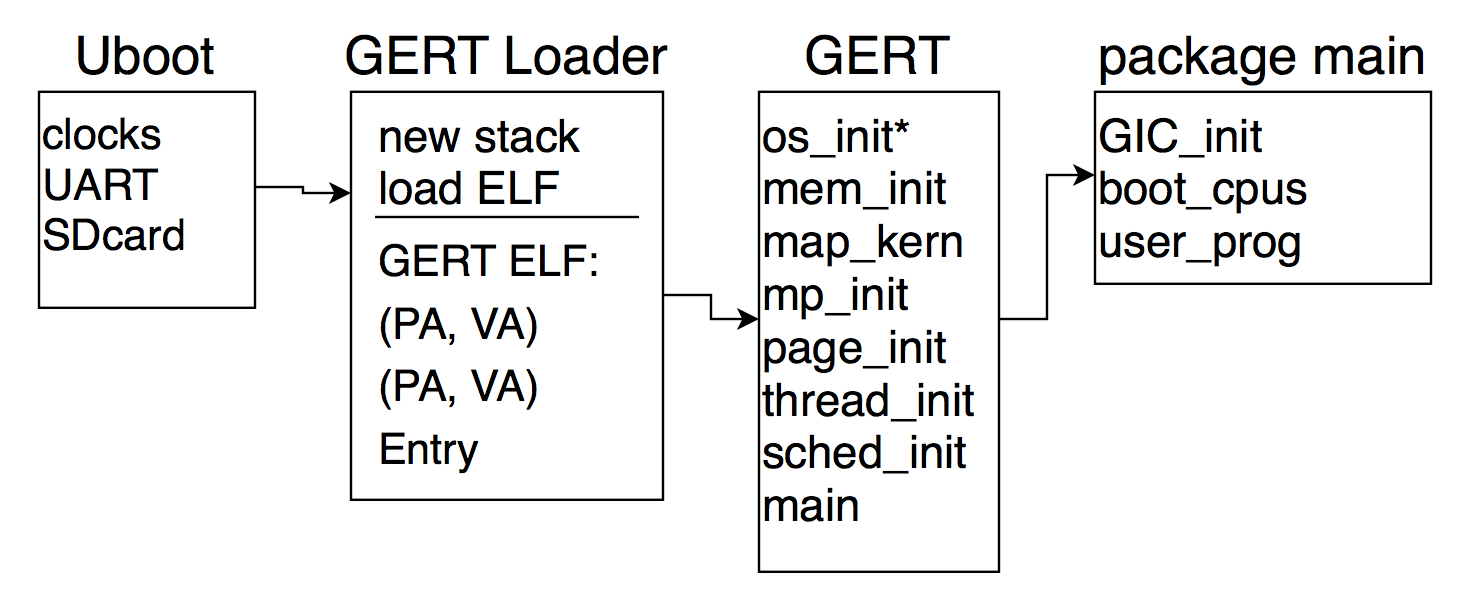
\includegraphics[scale=0.5]{boot_process}
\end{center}
  \caption{GERT Boot Process} \label{fig:boot}
\end{figure}

Even though Go code is compiled, it relies on a runtime to coordinate certain actions with the OS and support its concurrency model.
Timers, locks, and file descriptors are just a few of the OS abstractions that the runtime hinges on
in order to function at all. This means that getting compiled Go code to run bare metal on an SOC requires
more than just a boot loader, the Go runtime itself must be modified to work without any OS abstractions.
This poses a bootstrapping problem because any modifications made to the Go runtime's initialization
process must not inadvertently cause it to use an abstraction that does not yet exist. For example,
creating a new object with $make()$ \footnote{In Go, new objects are created with \textit{make}} during the boot process would be disastrous if the GC has not yet been initialized.
Modifying the Go runtime to boot on bare metal is tricky process because all additions should be made
in a non-destructive way that still preserves all of Go's useful primitives, including the standard library.


In observation of these constraints, GERT boots via a 3-step process as shown in  figure \ref{fig:boot}.
In step 1, u-boot is used to set up device clocks and load the code for step 2 off of an SD card. Step 2 prepares the
Go stack with arguments and environment variables before jumping into GERT. Step 3 runs inside of GERT and it
finishes the boot process by initializing virtual memory, threading, and interrupt handlers.




%%The first stage is the u-boot
%%bootloader, a common bootloader for embedded devices, which
%%configures the clocks and loads the second stage off of an SD card. The second
%%stage bootloader is a small C program which contains the entire GERT kernel ELF in its data section. This stage sets
%%up the inital Go stack and loads the GERT ELF into memory before jumping to its entry point. The third stage
%%of the bootloader lives inside GERT and is mostly written in Go, along with some Plan 9 assembly. It finishes the
%%boot process by initializing virtual memory, threading, and additional cpus.



%%Working off the
%%initial stack from stage 2, the stage 3 bootloader enumerates all of RAM into page tables and creates an idenity mapping
%%with a new stack before turning on the MMU. After this, a thread scheduler is setup and synchronization primitives, like
%%$futex()$ are enabled. Additional CPU's are booted in main after the Go runtime has finished initializing.

%%\section{System Specification}
%%GERT is written on a Freescale i.MX6 Quad SOC which implements the (32 bit) ARMv7a Cortex A9 MPCore architecture.
%%The SOC sits on a Wandboard Quad baseboard. The i.MX6 Quad has 2GB of RAM and a wealth of memory mapped peripherals.
%%Look at the memory map below. The rest of this chapter will discuss the implementation details of booting and
%%running the Go runtime bare-metal on this SOC.
%%
%%<memory map of imx6 here>
%%
%%<memory map of GERT here>

\section{Step 1 Bring Up}
Unlike desktop PCs, SOCs have no BIOS, so it is entirely the programmer's job to initialize device clocks
and power on essential peripherals like the memory controller. U-boot is a simple bootloader which abstracts
this laborious process for all of the SOCs which it supports. GERT uses it to chain load its own, more specialized,
bootloader. The u-boot loader is used to initialize device clocks and execute the GERT bootloader.


%%When the SOC is powered on, the program counter starts executing from ROM. The code in the ROM reads
%%u-boot into RAM and jumps into it. Unlike desktop PCs and laptops which use a BIOS to configure the
%%frequency dividers and RAM timings, the iMX6 has no such thing so u-boot does it instead.
%%U-boot programs the myriad of frequency dividers which are required
%%to run the i.MX6 at a frequency of 792MHz per core. After this, u-boot loads the GERT
%%kernel off the sdcard and into RAM at address 0x50000000. This address is specifically chosen because it
%%does not overlap with any ELF program headers of the GERT kernel which are loaded in stage 2. After
%%the stage 2 bootloader is in RAM, uboot jumps into it.

\section{Step 2 GERT Kernel Installation}
The GERT loader is a C program which sets up the initial Go stack and decompresses the Go kernel
ELF into RAM. GERT is compiled as a Linux Go program, so the Go runtime expects to find arguments
and environment variables in its initial stack. This is a convenient channel for passing
information; for example, the GERT loader uses this to pass the size of the GERT kernel.
GERT later uses this size to determine its location in memory and initialize virtual memory.

The link address of the GERT binary must be also adjusted on a per-SOC basis in order for the Go
runtime to avoid using inaccessible memory. By default, Go compiler links and loads at 0x0. This is incorrect
for most SOCs because they have reserved regions near that address. Fortunately, the Go compiler can
generate code at a different link addresses by passing in a link-time flag, so this is not a significant problem.

%%Much like Linux, the kernel of GERT is wrapped in a custom
%%bootloader. This is necessary because GERT is compiled as a user space
%%Linux program which expects a stack and the standard ELF auxiliary vectors to be present on
%%startup.
%%
%%By default, the Go compiler links all programs at address 0x0. This would normally
%%be a disaster for the i.MX6 because the first megabyte of RAM is either inaccessable
%%or reserved for peripherals. One solution around this is to simply turn on the MMU
%%in the stage 2 bootloader but this creates a headache with preserving page tables
%%across the transition to Go. An alternative, and much simpler, solution is to
%%just change the link address of the Go ELF. This is the preferred approach so
%%GERT's build system uses a link address of 0x10000000 for the Go runtime, which is the start of
%%RAM on the iMX6. After loading the Go binary into RAM, the stage 2 bootloader reserves
%%4kb of initial stack and jumps into GERT.


\section{Step 3 Go Runtime Setup}

The Go runtime forms the basis of GERT's functionality but it is not equipped to
run on bare metal. The final steps of the boot process are accomplished in Go. GERT
initializes the minimum set of OS abstractions
to be used by the Go runtime, before the runtime actually uses them. These abstractions are
virtual memory, thread scheduling, interrupt handling, timers, and booting secondary cores.

%%The thread scheduler and virtual memory system are statically initialized
%%in order to prevent Go runtime subsystems from running before the environment
%%is ready. At the beginning of execution, GERT is in a constrained
%%situation: Linux is not there but the Go runtime thinks it is. Specifically, there
%%is no scheduler, no virtual memory, no syscalls. Nothing but a 4kb stack
%%and the program counter. This is clearly inadequate for the Go runtime
%%to do anything but crash, so GERT creates all of these missing subsystems
%%,in Go, before the runtime actually uses them.


\subsection{Virtual Memory Setup}
\begin{figure}[h]
  \begin{subfigure}[t!]{0.5\textwidth}
 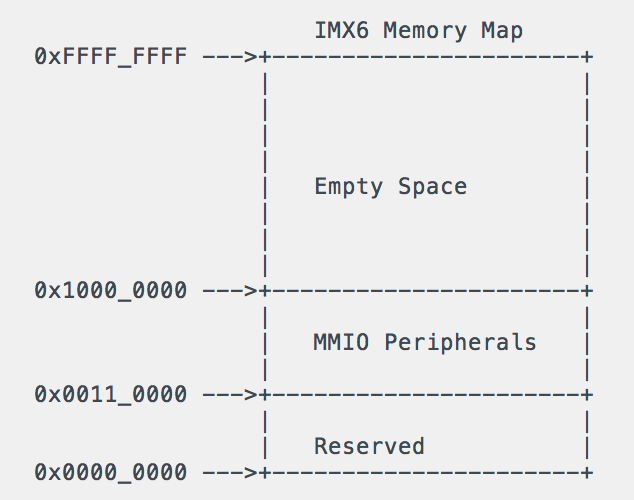
\includegraphics[scale=0.6]{imxmap}
  \end{subfigure}
  \begin{subfigure}[t!]{0.5\textwidth}
 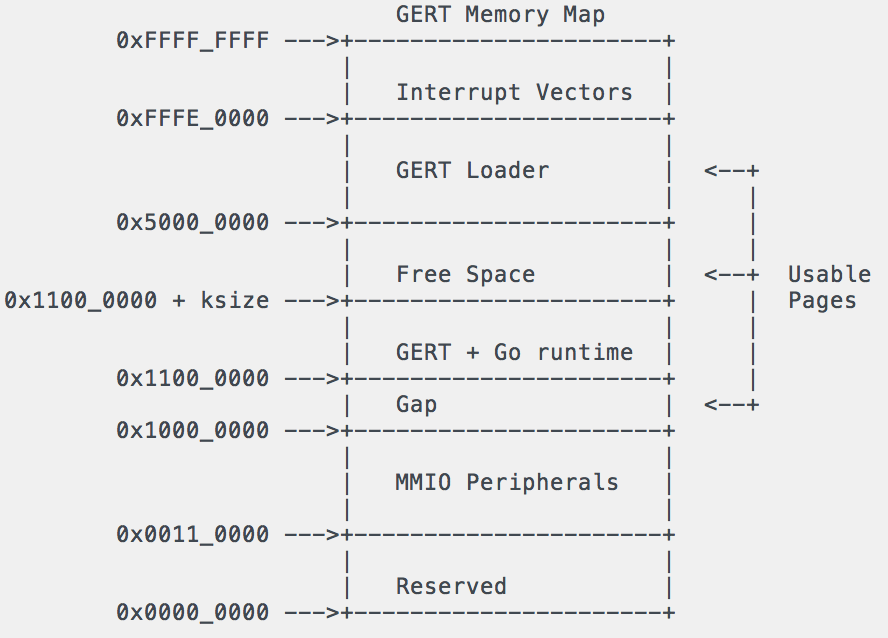
\includegraphics[scale=0.5]{gertmap}
  \end{subfigure}
  \caption{Memory Map Before and After Boot} \label{fig:gertmap}
\end{figure}

GERT needs to have virtual memory enabled so the Go runtime can function properly and so
GERT can manage available memory. Fig. \ref{fig:gertmap} shows the physical memory map
of an i.MX6 SOC before GERT is booted and after GERT has booted.
Even though the
runtime is linked at a high address, Go still requests memory inside the reserved regions of physical
memory so a virtual address must be mapped there. GERT also uses paging to create a virtually contiguous
address space which is easier to manage than a physically discontiguous address space. For example,
the Go runtime sometimes requests large chunks of continuous memory. It is possible that there is not
a large enough chunk of physical memory to return due to fragmentation of MMIO peripherals, but there
will be a big enough chunk in virtual memory. GERT also recycles the bootloader using virtual
memory by simply marking its occupied area as usable pages.

GERT uses 1MB page tables and it rarely has to reload them. GERT has no userspace or programs
that must be isolated from each other and the Go runtime only allocates memory infrequently
and in large chunks. This is the only time that GERT has to reload the page tables.
This static nature of GERT's memory space means that 4kb pages are unnecessary
and even costly because they incur a 2-level page translation \footnote{4kb paging in ARMv7a requires $2^11=4096$ entries in the L1 table and $2^8=256$ entries in each L2 table} , unlike 1MB pages which just require
a 1-level walk. By the time user code starts running in GERT, the runtime has nearly completed
all of its memory manipulation.

\subsection{Thread Scheduling and Trapframes}
\begin{figure}[h]
\begin{center}
  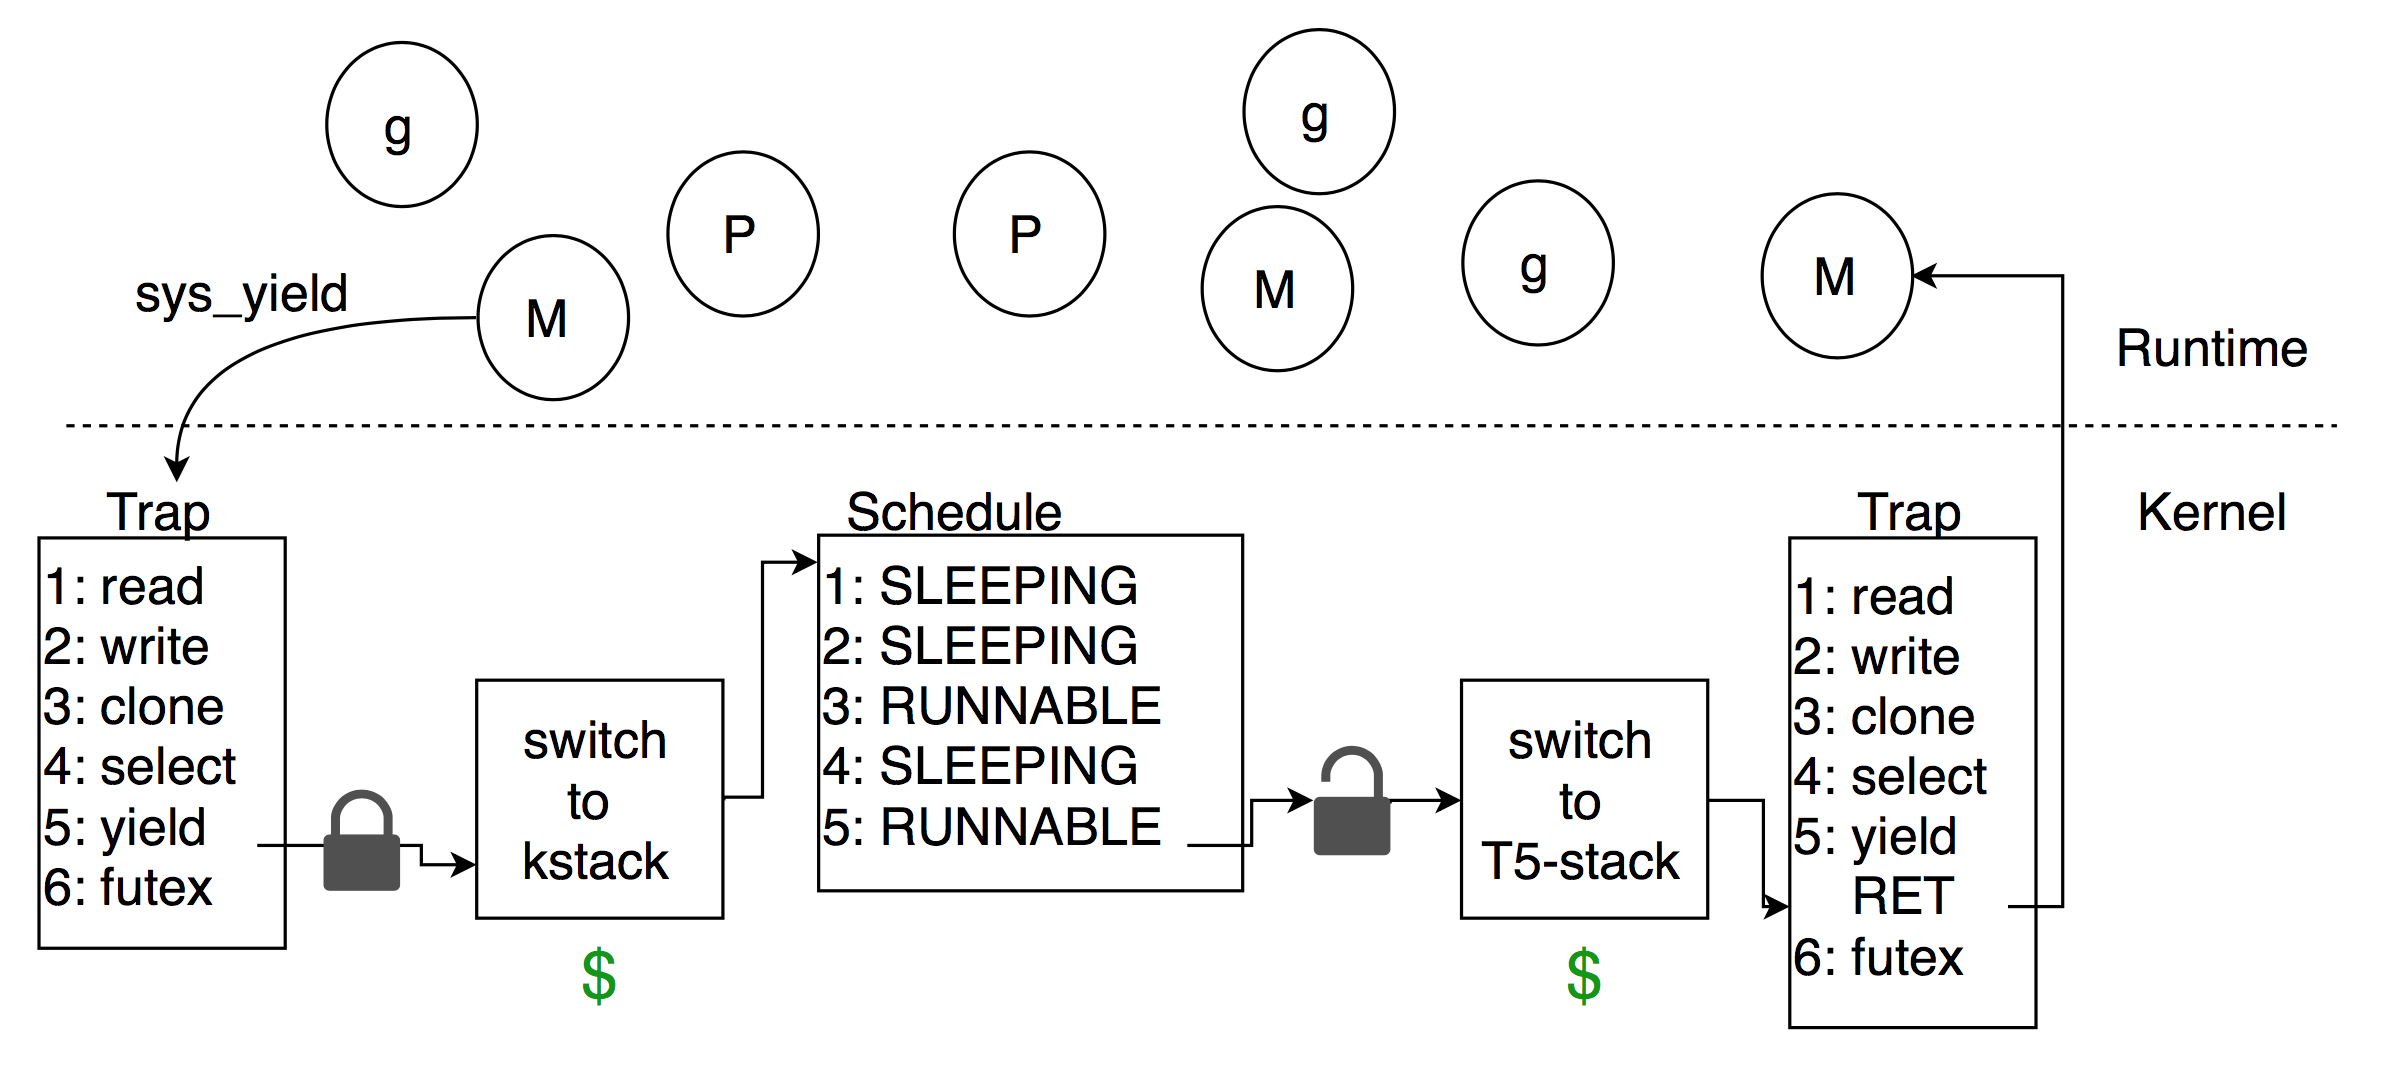
\includegraphics[scale=0.25]{syscall}
\end{center}
  \caption{Handling Go Runtime Syscalls} \label{fig:syscall}
\end{figure}

GERT models the entire Go runtime as a black box whose only entry and exit points
are through the syscalls it makes. This model is shown in \ref{fig:syscall} along with the
control flow of \textit{sys\_yield}, which invokes the GERT scheduler. To be clear, there is no such thing as a syscall in GERT;
it is a single-address space application that runs in privileged mode.
Whenever the Go runtime makes a syscall, the processor mode is not changed and a new page table
is not installed. Instead, every instance of the syscall instruction in the Go runtime has been
replaced with a function call to $trap$, the entry point into the GERT kernel.
While execution is in $trap$, the Go runtime believes
that the OS is servicing its syscall, but in actuality the blocked thread is still running Go code inside
the GERT kernel. The list of Linux syscalls that has to be re-implemented is shown in fig. \ref{fig:syscalls}.
All syscalls with an * are expensive because they cause a stack switch to the scheduler's stack.


\begin{figure} [h]
\begin{center}
  \begin{tabular}{ | l | l |}
    \hline
    Syscall & Used For \\ \hline
    exit & crash \\ \hline
    read & read from a file descriptor. All reads go to UART\\ \hline
    write & write to a file descriptor. All writes go to UART\\ \hline
    clone & spawn a new M\\ \hline
    *select & blocking read operation\\ \hline
    *yield & yield to scheduler\\ \hline
    mmap & allocate large chunks of memory\\ \hline
    *futex & wait for a condition to become true\\ \hline
    clock\_gettime & goroutine scheduling and time package\\ \hline
    getpid & runtime asks its pid\\ \hline
  \end{tabular}
\end{center}
  \caption{Linux Syscalls That Are Re-implemented in GERT}  \label{fig:syscalls}
\end{figure}

GERT also maintains data structures that track the state of Go threads
outside the runtime's knowledge. It is important that all state inside the GERT kernel is
allocated outside the Go runtime's knowledge either with global variables or the kernel's
static memory allocator. If this constraint is not observed, then it is possible for the garbage collector
to potentially recycle memory from the kernel.

Each thread in GERT has an id, status, futex address, and trapframe associated with it (\ref{fig:threadtrap}).
The trapframe records the state of all the registers and the location of the stack at
the time that the Go runtime made a syscall.

\begin{figure}[h]
  \begin{lstlisting}
type thread_t struct {
	tf       trapframe
	state    uint32
	futaddr  uintptr
	sleeptil timespec
	id       uint32
}
type trapframe struct {
	lr  uintptr
	sp  uintptr
	fp  uintptr
	r0  uint32
	r1  uint32
	r2  uint32
	r3  uint32
	r10 uint32
}
\end{lstlisting}

  \caption{Thread state and Trapframes} \label{fig:threadtrap}
\end{figure}

When threads go to sleep, the CPU stores their execution context in a trapframe.
When a thread is scheduled, the CPU restores the contents of the thread's last trap
frame and continues running the thread.

The futex, which stands for \textit{fast user space mutex}, is a useful building block
that the Linux kernel (and now GERT) provides to help with locking. Linux user space programs can use
it to wait until a certain condition becomes true, and the Go runtime uses it extensively
to monitor elapsed time and wake sleeping threads.


\subsection{Interrupts}
\begin{figure}[h]
\begin{center}
  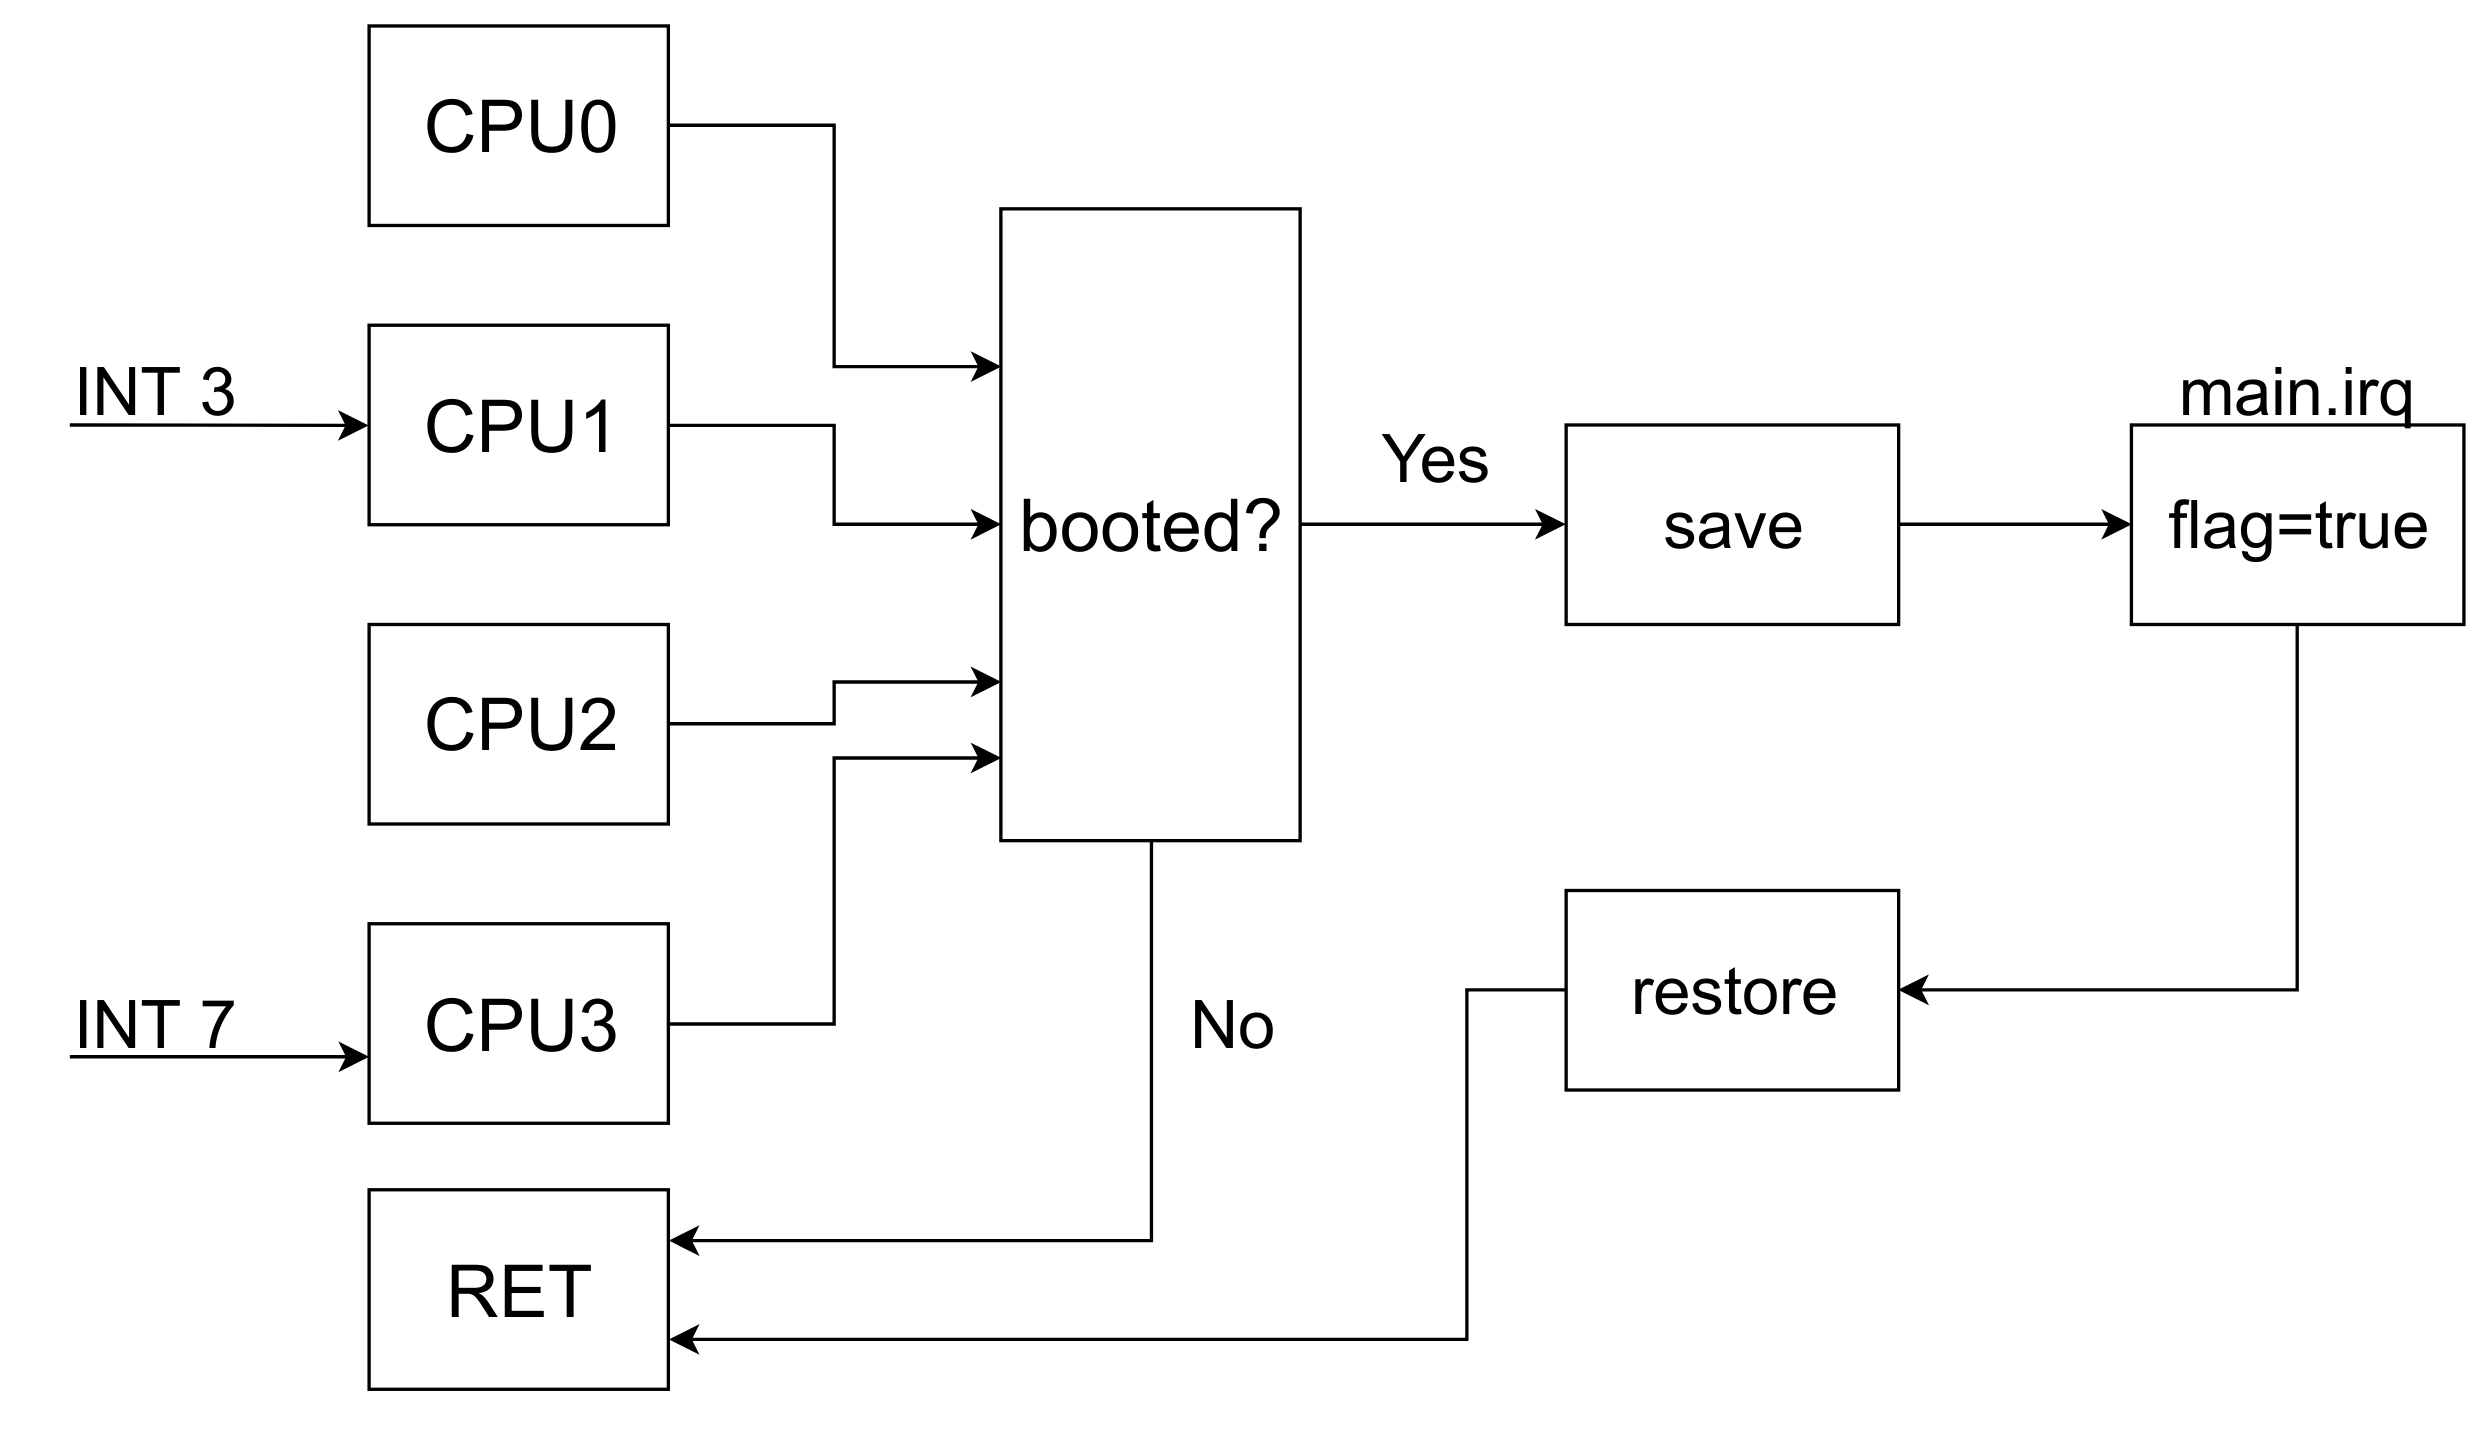
\includegraphics[scale=0.1]{interrupt}
\end{center}
  \caption{Handling Interrupts in GERT} \label{fig:interrupt}
\end{figure}

The interrupt handling process in GERT is explicitly designed so
that interrupts can always be serviced, even when Go's garbage collector
is running. To achieve this design, GERT puts some restrictions on the Go code
in an interrupt handler, as described below.

When a GC cycle runs, it can potentially stop the world and
prevent any Go code from executing. On a desktop OS it might be OK to disable
interrupts during a GC cycle because it is infrequent, but on an embedded system
interrupts could occur at any time, even while the world is
stopped. GERT allows interrupts to trigger at all times by assuming that the
interrupt handler does not perform any blocking operations. A block diagram
of the GERT interrupt process is shown in fig. \ref{fig:interrupt}.

GERT's interrupt handlers are written in Go and they execute on dedicated interrupt stacks.
When GERT receives an interrupt, the target processor
automatically switches its stack to the interrupt stack and then the GERT interrupt handler saves its old execution context onto the new stack.
Before proceeding any further, the interrupt handler checks a boolean flag to see if GERT has fully booted yet. This is important
for preventing unintentional Go code from executing while the memory map is still undefined.
While secretly executing on the interrupt stack, the processor can run any Go code
as long as it does not invoke the Go scheduler. This is because the Go runtime is unaware
of any interrupt code that can possibly run so it does not maintain any G's or M's to
run it. Thus, from the view of the Go runtime, the interrupt handler is running on an unknown secret stack which attaches itself
to whichever M was interrupted.

Interrupt handlers in GERT should not execute blocking operations or allocate memory from the Go heap \footnote{Go maintains a pool of free memory from which it allocates new objects. Most computer programs have a heap, not just Go programs.}.
The garbage collector is unaware of the hidden interrupt stacks so any heap-allocated objects on the stacks
will become memory leaks because the GC will never scan it. Fortunately, allocating heap objects in the interrupt
handler will cause a panic because \textit{make()}, and many other blocking operations, need to acquire
a lock from the runtime. This is dangerous because the runtime keeps track of which Ms are holding locks
and interrupt code can violate its beliefs and cause an unrecoverable panic.

Interrupt
routines should be short and execute quickly in order to avoid missing sequential
interrupts. This limits acceptable operations in an interrupt handler to toggling global boolean
flags and non-blocking reads/writes to memory. A typical GERT program is unaffected by these constraints
because it can use a goroutine to monitor a flag which is only toggled in the interrupt handler.

\subsection{Keeping Time}

Go needs a timer to schedule goroutines properly. GERT uses the 64bit ARM global timer which
is part of the general ARMv7a architecture \cite{ddi0406}. In the timer, each tick is about 2$ns$ so this means it will
not overflow for 1169 years. This means that GERT does not need a special timer interrupt to know when the
counter rolls over. The current value of the timer is returned whenever the Go runtime calls
the \textit{clock\_gettime()} syscall by reading from its MMIO address.

\subsection{Booting Secondary CPUs}

GERT boots auxiliary CPU's in two stages. After power on, the primary CPU starts executing at address 0x0 but the
secondary CPU's are held in a \textit{wait for interrupt} state. GERT creates an initial 4kb stack for each additional CPU,
which also doubles as its interrupt stack, before instructing them into a holding pen. The secondary CPU's
stay in the holding pen while GERT and the Go runtime finish booting because the virtual memory map is
in a state of flux. After GERT has booted, the user must call \textit{Release()} which causes the secondary CPU's
to reload their page tables and exit the holding pen into the GERT scheduler. Now the secondary CPU's
can each run Go threads normally.


